\documentclass[14pt]{extbook}
\usepackage{multicol, enumerate, enumitem, hyperref, color, soul, setspace, parskip, fancyhdr} %General Packages
\usepackage{amssymb, amsthm, amsmath, latexsym, units, mathtools} %Math Packages
\everymath{\displaystyle} %All math in Display Style
% Packages with additional options
\usepackage[headsep=0.5cm,headheight=12pt, left=1 in,right= 1 in,top= 1 in,bottom= 1 in]{geometry}
\usepackage[usenames,dvipsnames]{xcolor}
\usepackage{dashrule}  % Package to use the command below to create lines between items
\newcommand{\litem}[1]{\item#1\hspace*{-1cm}\rule{\textwidth}{0.4pt}}
\pagestyle{fancy}
\lhead{Progress Quiz 7}
\chead{}
\rhead{Version C}
\lfoot{4173-5738}
\cfoot{}
\rfoot{Spring 2021}
\begin{document}

\begin{enumerate}
\litem{
Solve the radical equation below. Then, choose the interval(s) that the solution(s) belongs to.\[ \sqrt{8 x^2 + 24} - \sqrt{-28 x} = 0 \]\begin{enumerate}[label=\Alph*.]
\item \( x \in [-1.94,-1.24] \)
\item \( x_1 \in [1.27, 1.89] \text{ and } x_2 \in [-1,4] \)
\item \( \text{All solutions lead to invalid or complex values in the equation.} \)
\item \( x \in [-2.29,-1.98] \)
\item \( x_1 \in [-2.29, -1.98] \text{ and } x_2 \in [-1.5,-0.5] \)

\end{enumerate} }
\litem{
Choose the equation of the function graphed below.
\begin{center}
    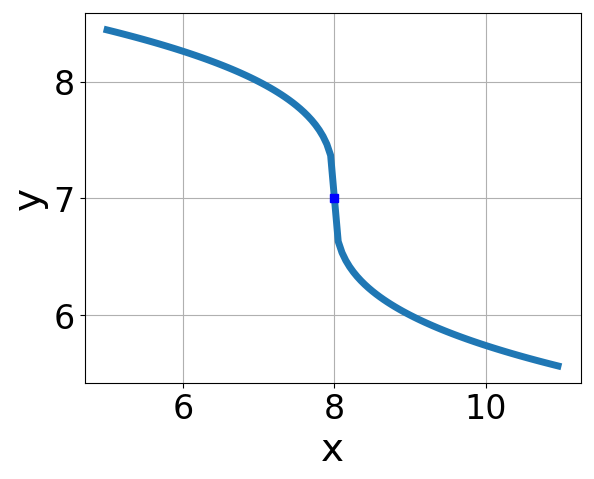
\includegraphics[width=0.5\textwidth]{../Figures/radicalGraphToEquationC.png}
\end{center}
\begin{enumerate}[label=\Alph*.]
\item \( f(x) = - \sqrt{x + 8} + 7 \)
\item \( f(x) = \sqrt{x + 8} + 7 \)
\item \( f(x) = \sqrt{x - 8} + 7 \)
\item \( f(x) = - \sqrt{x - 8} + 7 \)
\item \( \text{None of the above} \)

\end{enumerate} }
\litem{
Solve the radical equation below. Then, choose the interval(s) that the solution(s) belongs to.\[ \sqrt{15 x^2 - 48} - \sqrt{-22 x} = 0 \]\begin{enumerate}[label=\Alph*.]
\item \( x_1 \in [-3.67, -0.67] \text{ and } x_2 \in [0.75,1.23] \)
\item \( x_1 \in [-0.8, 4.2] \text{ and } x_2 \in [1.53,3.1] \)
\item \( x \in [-0.8,4.2] \)
\item \( \text{All solutions lead to invalid or complex values in the equation.} \)
\item \( x \in [-3.67,-0.67] \)

\end{enumerate} }
\litem{
Choose the graph of the equation below.\[ f(x) = - \sqrt[3]{x + 8} + 5 \]\begin{enumerate}[label=\Alph*.]
\begin{multicols}{2}\item 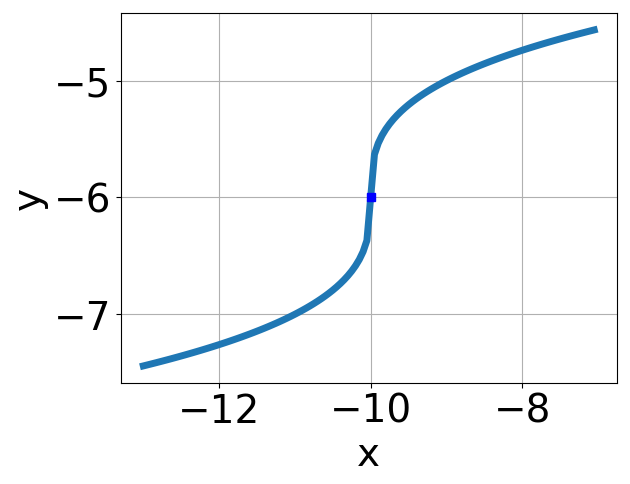
\includegraphics[width = 0.3\textwidth]{../Figures/radicalEquationToGraphAC.png}\item 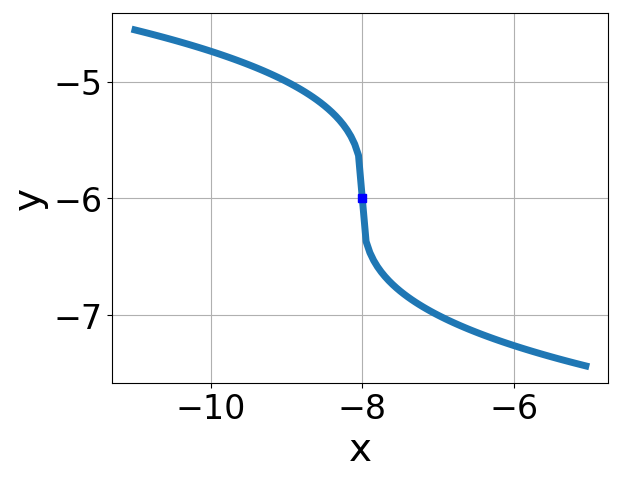
\includegraphics[width = 0.3\textwidth]{../Figures/radicalEquationToGraphBC.png}\item 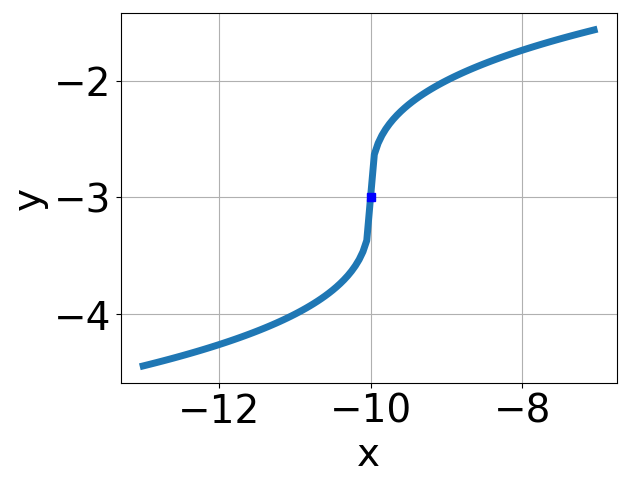
\includegraphics[width = 0.3\textwidth]{../Figures/radicalEquationToGraphCC.png}\item 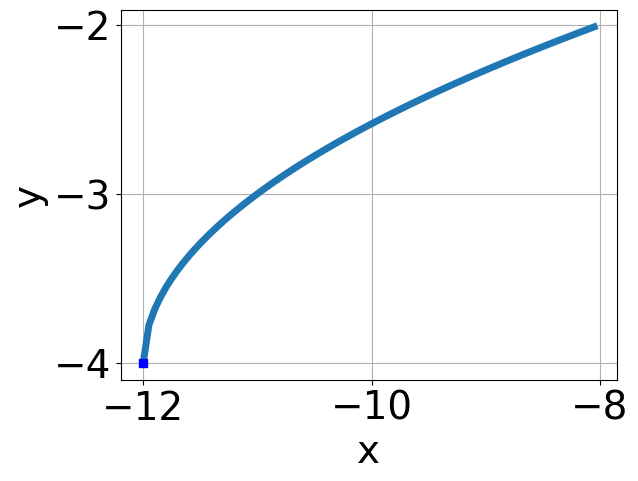
\includegraphics[width = 0.3\textwidth]{../Figures/radicalEquationToGraphDC.png}\end{multicols}\item None of the above.
\end{enumerate} }
\litem{
Solve the radical equation below. Then, choose the interval(s) that the solution(s) belongs to.\[ \sqrt{-7 x + 5} - \sqrt{8 x + 2} = 0 \]\begin{enumerate}[label=\Alph*.]
\item \( x_1 \in [-0.3, -0.08] \text{ and } x_2 \in [-0.29,1.71] \)
\item \( x_1 \in [0.1, 0.46] \text{ and } x_2 \in [-0.29,1.71] \)
\item \( \text{All solutions lead to invalid or complex values in the equation.} \)
\item \( x \in [0.1,0.46] \)
\item \( x \in [0.3,0.57] \)

\end{enumerate} }
\litem{
Choose the graph of the equation below.\[ f(x) = \sqrt{x - 12} - 4 \]\begin{enumerate}[label=\Alph*.]
\begin{multicols}{2}\item 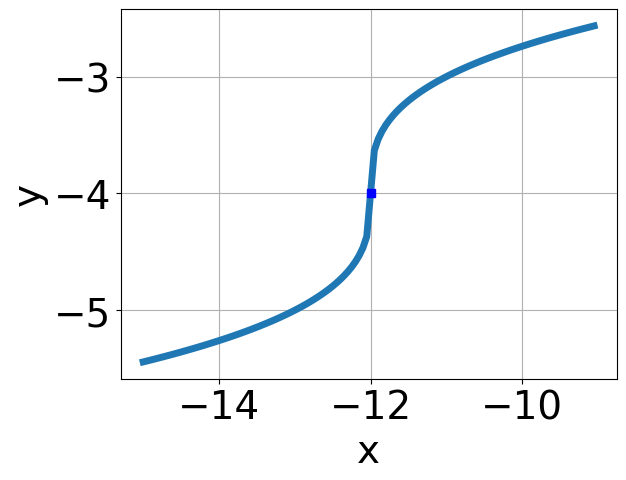
\includegraphics[width = 0.3\textwidth]{../Figures/radicalEquationToGraphCopyAC.png}\item 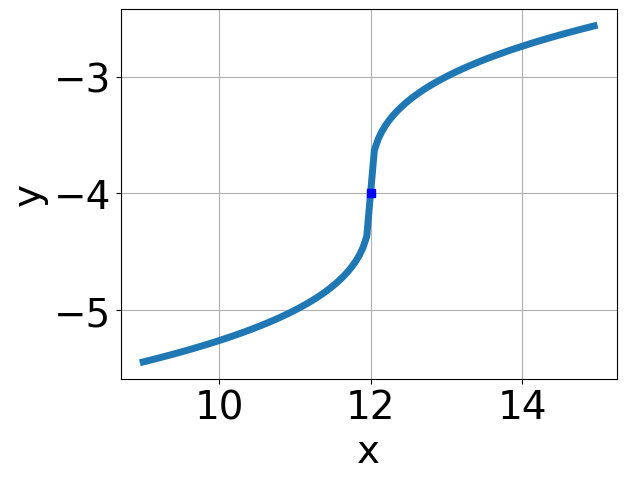
\includegraphics[width = 0.3\textwidth]{../Figures/radicalEquationToGraphCopyBC.png}\item 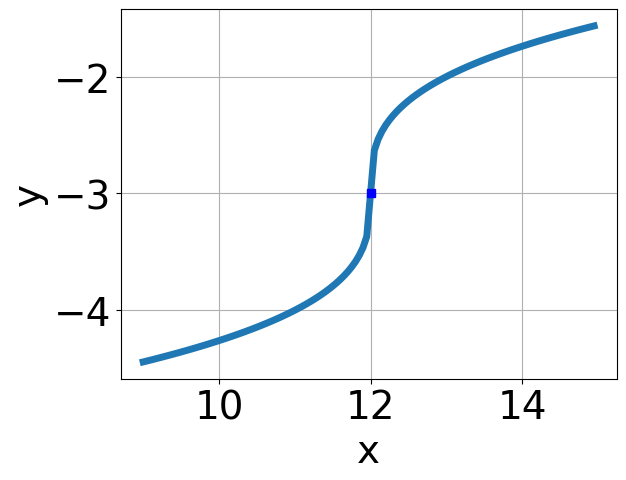
\includegraphics[width = 0.3\textwidth]{../Figures/radicalEquationToGraphCopyCC.png}\item 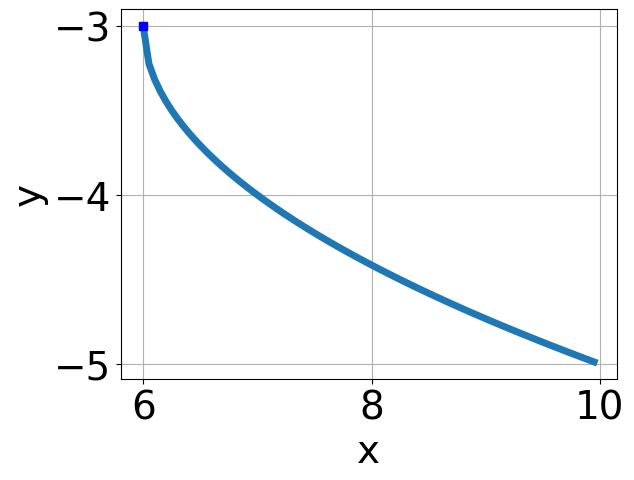
\includegraphics[width = 0.3\textwidth]{../Figures/radicalEquationToGraphCopyDC.png}\end{multicols}\item None of the above.
\end{enumerate} }
\litem{
What is the domain of the function below?\[ f(x) = \sqrt[6]{-5 x - 7} \]\begin{enumerate}[label=\Alph*.]
\item \( [a, \infty), \text{where } a \in [-4.3, -0.9] \)
\item \( (-\infty, a], \text{where } a \in [-1.13, -0.68] \)
\item \( (-\infty, \infty) \)
\item \( (-\infty, a], \text{ where } a \in [-1.75, -1.32] \)
\item \( [a, \infty), \text{where } a \in [-1.2, -0.6] \)

\end{enumerate} }
\litem{
What is the domain of the function below?\[ f(x) = \sqrt[8]{-6 x + 3} \]\begin{enumerate}[label=\Alph*.]
\item \( [a, \infty), \text{where } a \in [-1.5, 1.9] \)
\item \( [a, \infty), \text{where } a \in [0.7, 4] \)
\item \( (-\infty, a], \text{ where } a \in [-0.5, 1.5] \)
\item \( (-\infty, a], \text{where } a \in [2, 8] \)
\item \( (-\infty, \infty) \)

\end{enumerate} }
\litem{
Solve the radical equation below. Then, choose the interval(s) that the solution(s) belongs to.\[ \sqrt{-8 x + 5} - \sqrt{-9 x - 8} = 0 \]\begin{enumerate}[label=\Alph*.]
\item \( x_1 \in [-1.6, 0.5] \text{ and } x_2 \in [0.62,6.62] \)
\item \( x_1 \in [-15.3, -11.9] \text{ and } x_2 \in [0.62,6.62] \)
\item \( x \in [-15.3,-11.9] \)
\item \( x \in [1.7,3.8] \)
\item \( \text{All solutions lead to invalid or complex values in the equation.} \)

\end{enumerate} }
\litem{
Choose the equation of the function graphed below.
\begin{center}
    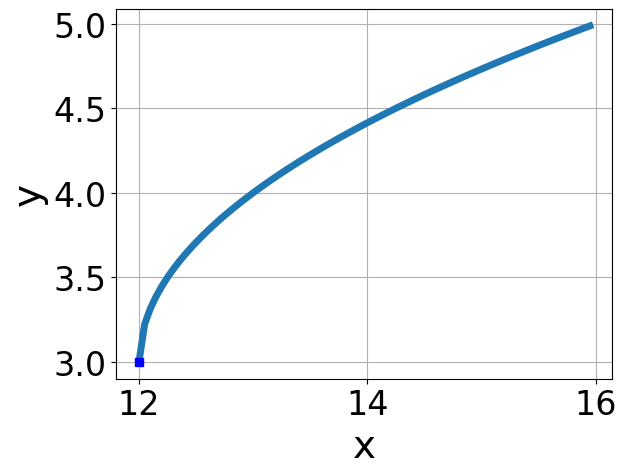
\includegraphics[width=0.5\textwidth]{../Figures/radicalGraphToEquationCopyC.png}
\end{center}
\begin{enumerate}[label=\Alph*.]
\item \( f(x) = \sqrt{x + 14} + 7 \)
\item \( f(x) = - \sqrt{x + 14} + 7 \)
\item \( f(x) = \sqrt{x - 14} + 7 \)
\item \( f(x) = - \sqrt{x - 14} + 7 \)
\item \( \text{None of the above} \)

\end{enumerate} }
\end{enumerate}

\end{document}